% WSCG sample document
%
% based on Gabriel Zachmann's sample
% http://zach.in.tu-clausthal.de/latex/
%
% modified Apr 2012 to match WSCG Word template
%
\documentclass[twoside,twocolumn,10pt]{article}



%%%%%%%%%%%%%%%%%%%%%%%%%%%%%%%%%%%%%%%%%%%%%%%%%%%%%%%%%%%%%%%%%%%%%%%%%%%%%
%                             Packages

\usepackage{wscg}           % includes a number of other packages (e.g., myalgorithm)
\RequirePackage{ifpdf}
\ifpdf
 \RequirePackage[pdftex]{graphicx}
 \RequirePackage[pdftex]{color}
\else
 \RequirePackage[dvips,draft]{graphicx}
 \RequirePackage[dvips]{color}
\fi
\usepackage{subfig}

\usepackage{nopageno}       % no page numbers at all; uncomment for final version
\usepackage{graphicx}
\usepackage[justification=centering]{caption}
\usepackage{amsmath}
\usepackage[linesnumbered,ruled]{algorithm2e}
\usepackage[english]{babel}
%\usepackage[utf8]{inputenc}
\usepackage{enumitem}
%%%%%%%%%%%%%%%%%%%%%%%%%%%%%%%%%%%%%%%%%%%%%%%%%%%%%%%%%%%%%%%%%%%%%%%%%%%%%
%                                Title

\title{MAELab: a framework to automatize landmark estimation}

\author{
  \hspace{-0.1\textwidth}
  \parbox{0.2\textwidth}{\centering
    LE Van \\
    Linh\\[1mm]
LaBRI-CNRS 5800\\
ITDLU, Dalat Univ-V
linhlv@dlu.edu.vn/ van-linh.le@labri.fr
}
\hspace{0.02\textwidth}
\parbox{0.2\textwidth}{\centering
BEURTON-AIMAR Marie\\[1mm]
LaBRI-CNRS 5800\\
Bordeaux University\\
33400 Talence-F\\
beurton@labri.fr
}
\hspace{0.02\textwidth}
\parbox{0.25\textwidth}{\centering
KRAHENBUHL \\Adrien\\[1mm]
LaBRI-CNRS 5800\\
Bordeaux University\\
33400 Talence-F\\
adrien.krahenbuhl@labri.fr
}
\hspace{0.02\textwidth}
\parbox{0.18\textwidth}{\centering
PARISEY\\ Nicolas\\[1mm]
IGEPP\\
INRA 1349\\
35653 Le Rheu-F\\
nparisey@rennes.inra.fr
}
}

%%%%%%%%%%%%%%%%%%%%%%%%%%%%%%%%%%%%%%%%%%%%%%%%%%%%%%%%%%%%%%%%%%%%%%%%%%%%%
%                          Hyperref


% no hyperlinks
\usepackage{url}
\urlstyle{tt}

% Donald Arsenau's fix for missing kerning of "//" and ":/"
\makeatletter
\def\Uslash{\mathbin{\mathchar`\/}\@ifnextchar{/}{\kern-.15em}{}}
\g@addto@macro\UrlSpecials{\do \/ {\Uslash}}
\def\Ucolon{\mathbin{\mathchar`:}\@ifnextchar{/}{\kern-.1em}{}}
\g@addto@macro\UrlSpecials{\do : {\Ucolon}}
\makeatother




%%%%%%%%%%%%%%%%%%%%%%%%%%%%%%%%%%%%%%%%%%%%%%%%%%%%%%%%%%%%%%%%%%%%%%%%%%%%%
%                                Document


\begin{document}

\twocolumn[{\csname @twocolumnfalse\endcsname

\maketitle  % full width title


\begin{abstract}
In biology, the morphometric analysis is widely used to analyze the inter-organisms variations.
It allows to classify and to determine the evolution of an organism's family.
The morphometric methods consider features such as shape, structure, color, or size of the studied objects.
In previous works \cite{leestimating}, we have analyzed beetle mandibles by using the centroid as feature, in order to classify the beetles.
We have shown that the Probabilistic Hough Transform (PHT) is an efficient unsupervised method to compute the centroid.
This paper proposes a new approach to precisely estimate the landmark geometry, points of interest defined by biologists on the mandible contours.
In order to automatically register the landmarks on different mandibles, we defined patches around manual landmarks of the reference image.
Each patch is described by computing its SIFT descriptor.
Considering a query image, we apply a registration step performed by an Iterative Principal Component Analysis which identify the rotation and translation parameters.
Then, the patches on the query image are identified and the SIFT descriptors computed.
The biologists have collected $293$ beetles to provide two sets of mandible images separated into left and right side.
The experiments show that, depending on the position of the landmarks on the mandible contour, the performance can go up to $98\%$ of good detection.
The complete workflow is implemented in the MAELab framework, freely available as library on GitHub.
\end{abstract}

\subsection*{Keywords}
Morphology, image registration, SIFT descriptor, beetle, mandible.
\vspace*{1.0\baselineskip}
}]



%%%%%%%%%%%%%%%%%%%%%%%%%%%%%%%%%%%%%%%%%%%%%%%%%%%%%%%%%%%%%%%%%%%%%%%%%%%%%


\section{Introduction}

\copyrightspace
 Phenotype of beetle species are characterized by informations like age, sex, morphological criteria or environmental parameters.
 Biologists are used to proceed to manual measurements in case of analysis at macro level as for example tissues or animal members \cite{houle2003automated} \cite{bromiley2014semi}.
 They can directly measure the geometrical characteristics of elements on the body of the animal: length, width, diameter, angles, etc.
 Another way to obtain morphological measures is to take pictures of the members and to apply image processing algorithms.
 In order to evaluate a population of beetles from Brittany lands, a collection of $293$ beetles has been established.
 For each beetle, biologists took images of the left and right mandibles (see Fig. \ref{figparts}) and a set of landmarks has been manually determined by experts.
 A morphometric landmark is a specific points, directly linked to the animal anatomy.
 The landmarks are used in many domains, not only in biological studies.
 It is an application field in image processing \cite{li09} that appears in works of computer vision, mainly in face recognition \cite{zhang2014facial} but also in human orthodontic \cite{favaedi2010cephalometric} or morphometric
 analysis \cite{bec03}.

\begin{figure}[htbp]
\centering
\subfloat[Left mandible]{\label{figrbox2}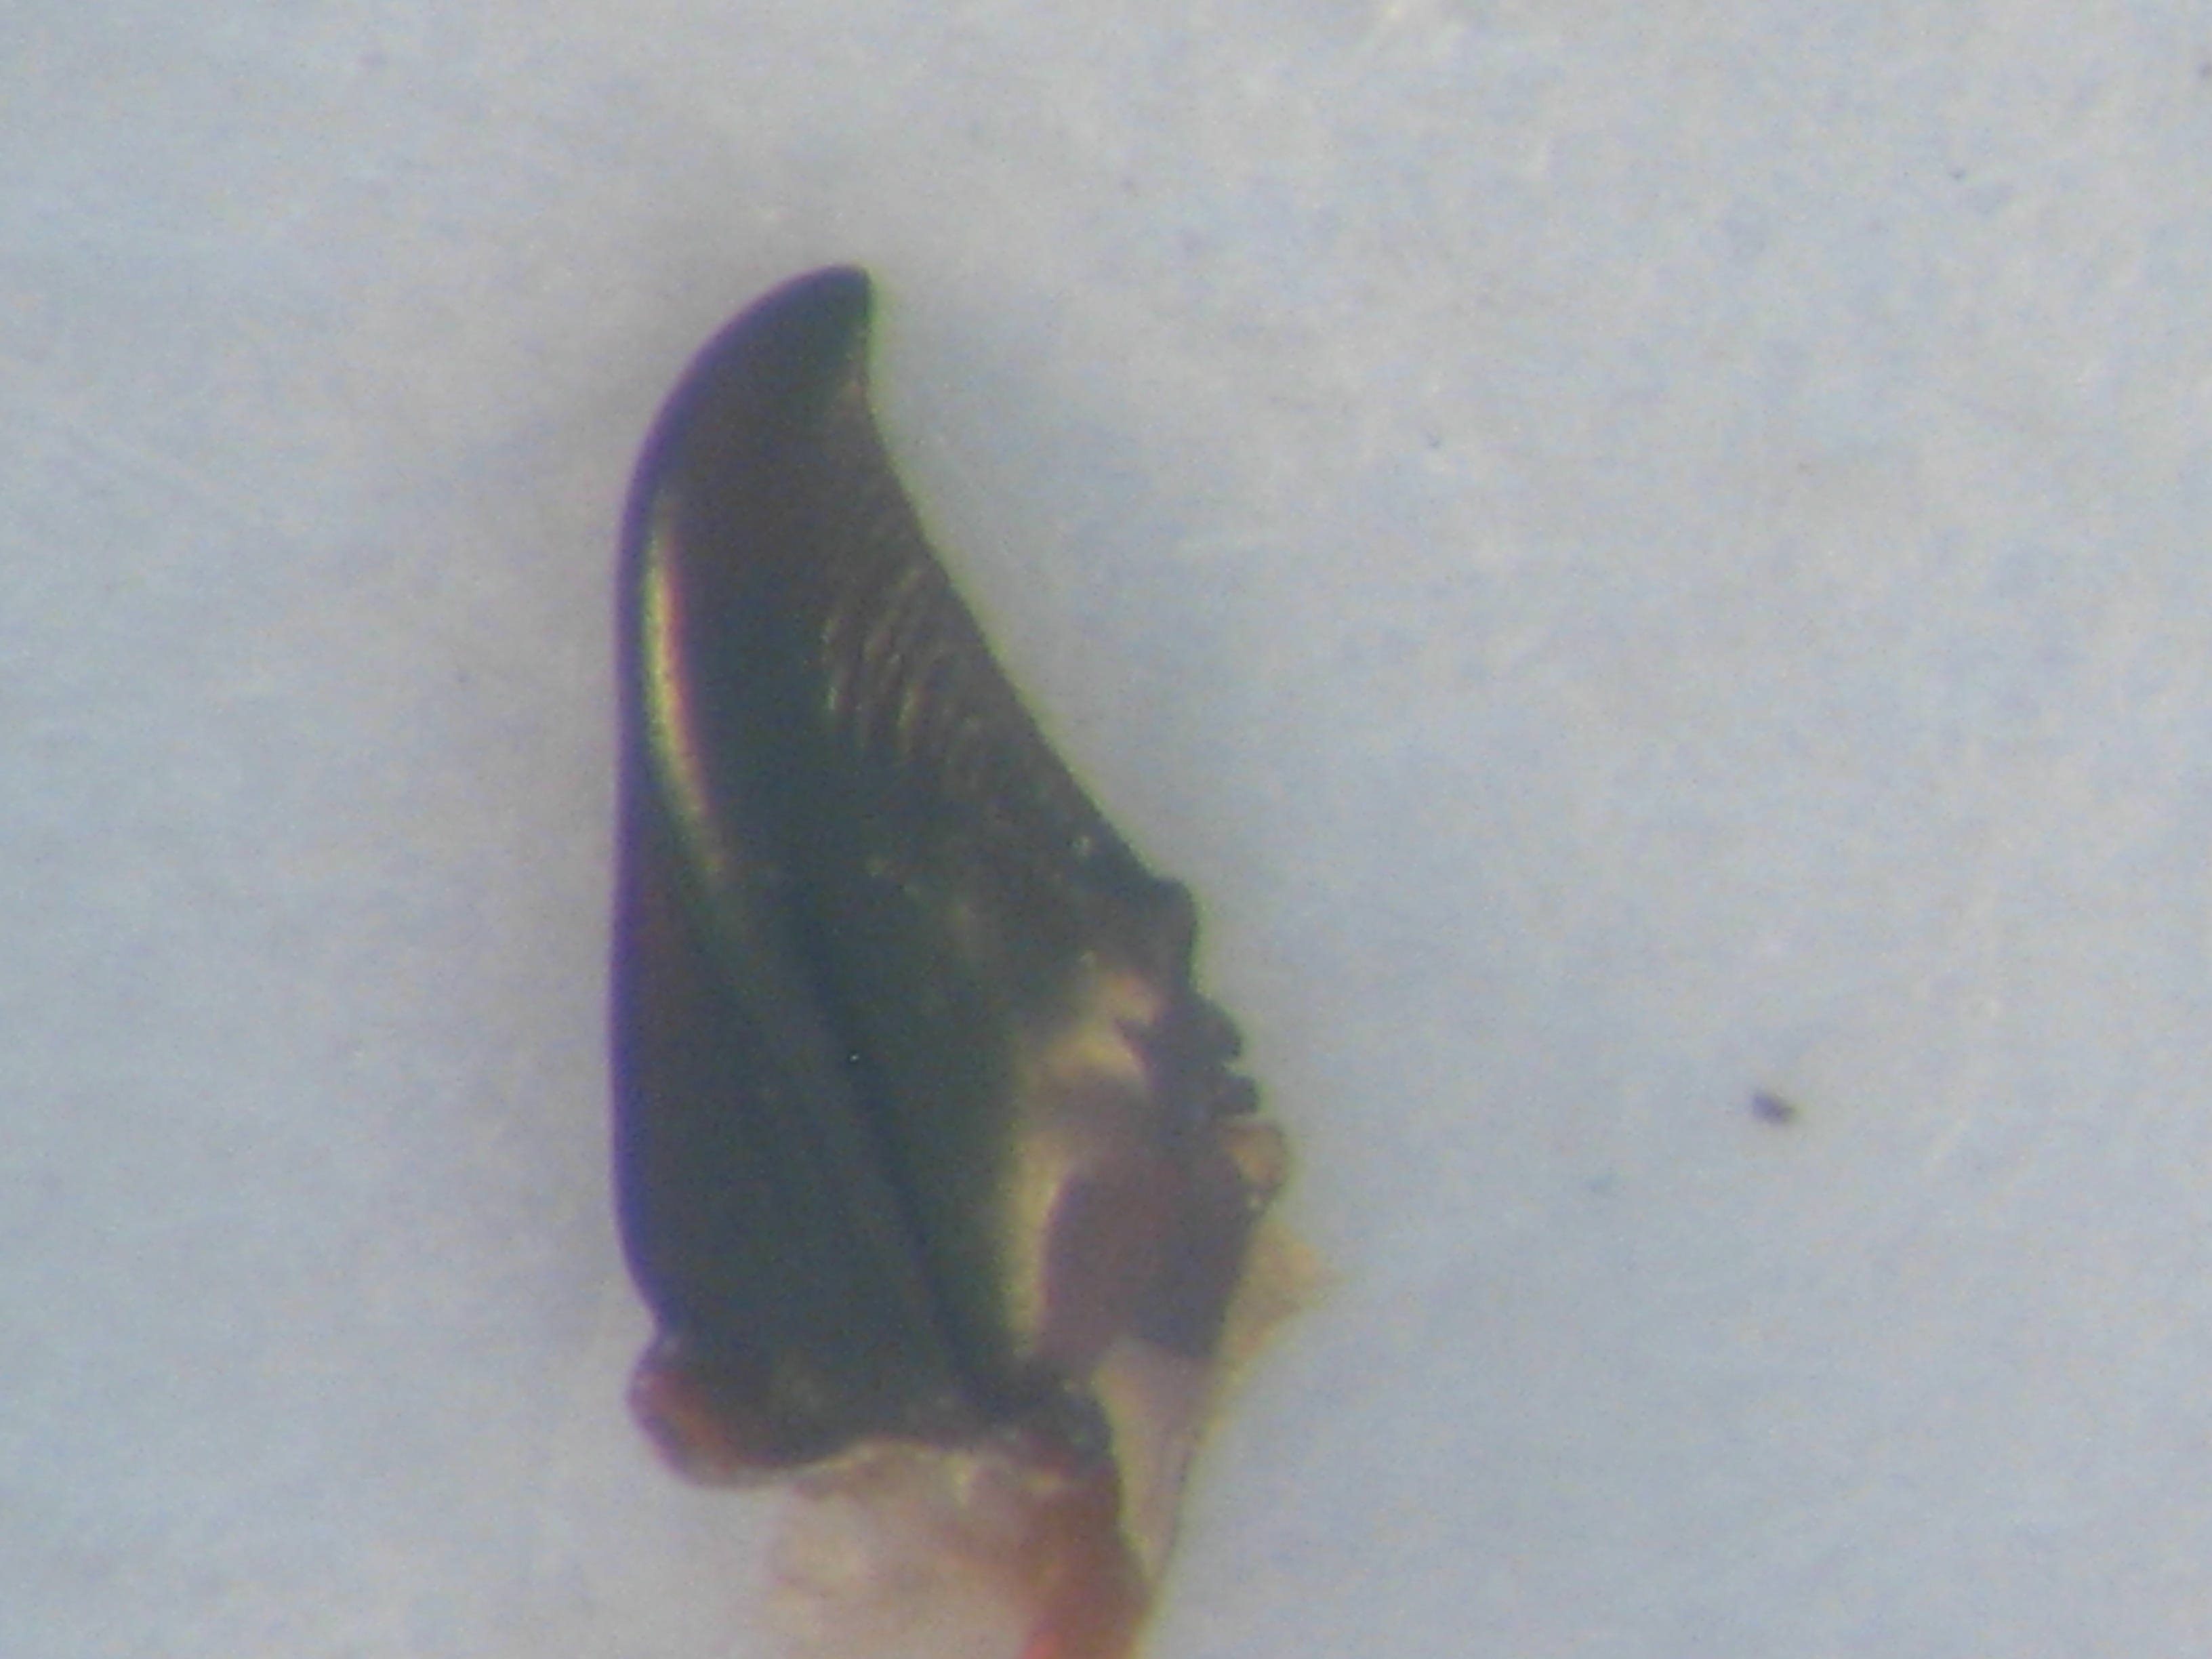
\includegraphics[width=0.23\textwidth]{./images/lm}}~~
\subfloat[Right mandible]{\label{figrbox1}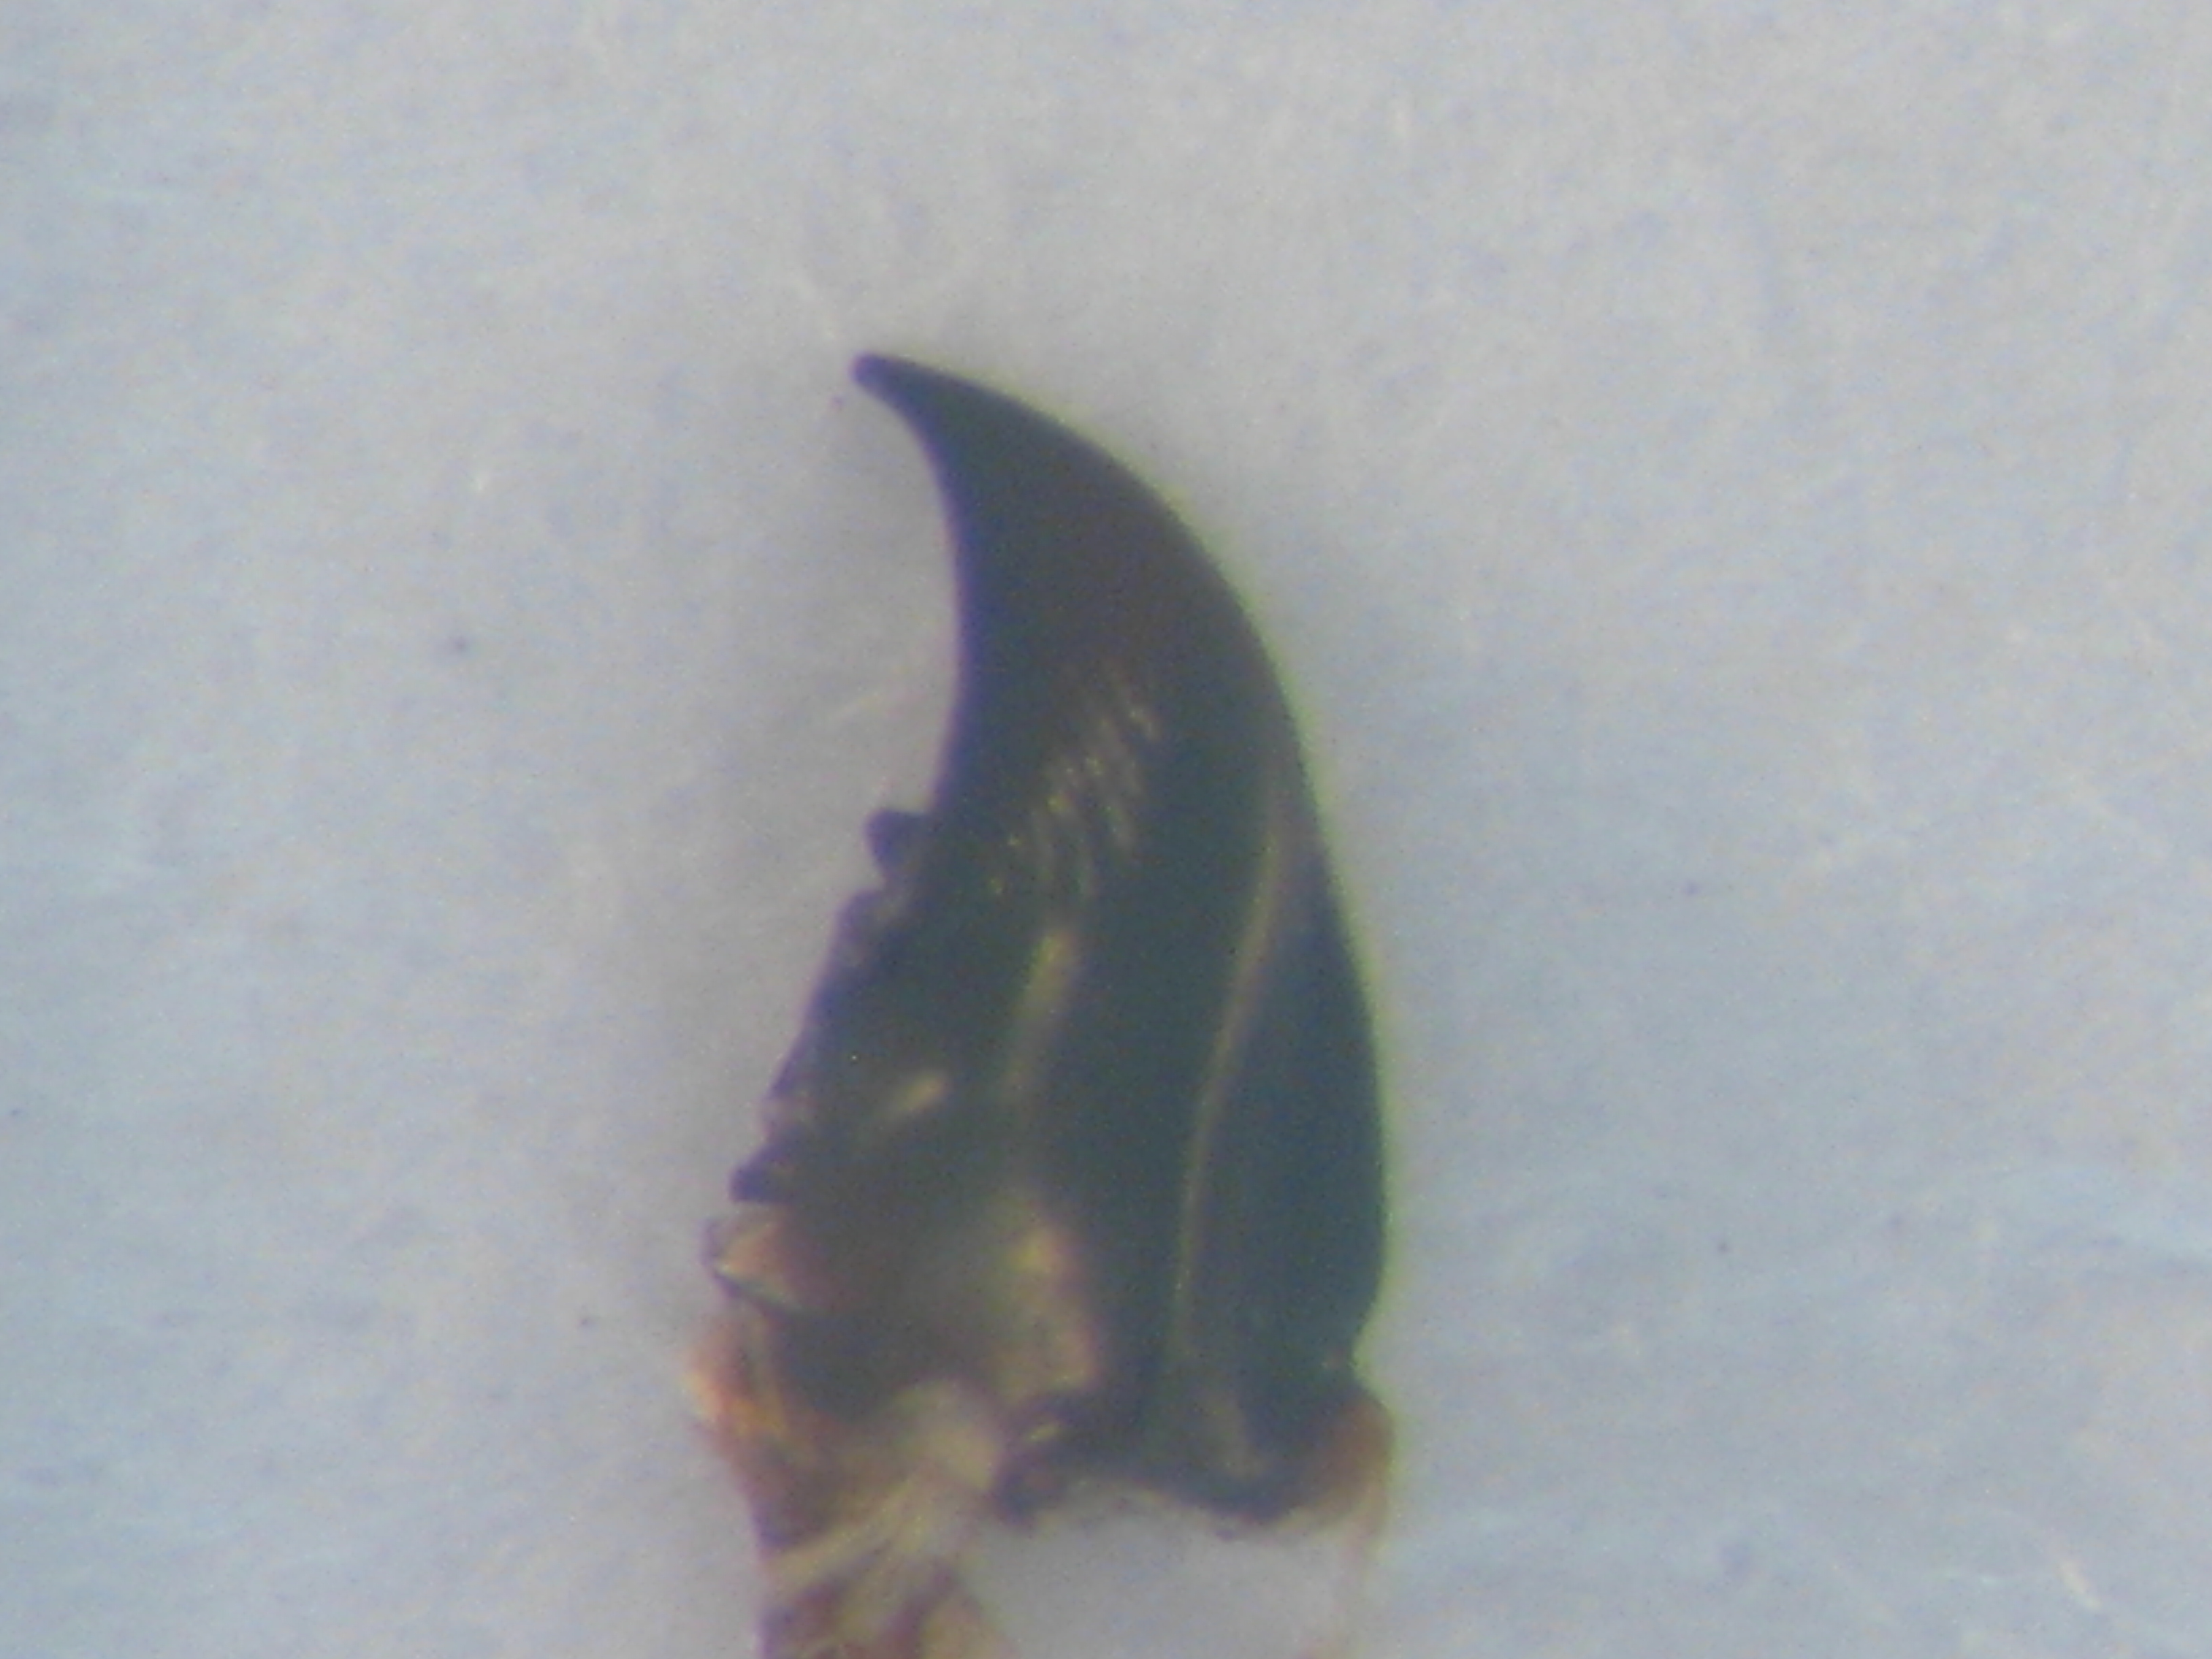
\includegraphics[width=0.23\textwidth]{./images/rm}}
\caption{The two mandibles of a beetle captured by biologists.}
\label{figparts}
\end{figure}

In this paper, we focus on the automatic identification of landmarks in 2D mandible images.
The proposed method consists of three main steps: a segmentation of the mandible based on the Canny algorithm, an Iterative Principal
Component Analysis to register a query image on a model image, and finally a landmark estimation on the query image by comparison of SIFT descriptors.
Section \ref{sec:method} presents the complete workflow then section \ref{sec:experiments} details the experiments and analyzes the results.


%%%%%%%%%%%%%%%%%%%%%%%%%%%%%%%%%%%%%%%%%%%%%%%%%%%%%%%%%%%%%%%%%%%%%%%%%%%%%
\section{Method}
\label{sec:method}

The addressed problem is the automatic detection of morphologic landmarks on mandible pictures to replace the manual operation made by an expert operator.
We details hereafter a workflow (resumed Fig. \ref{fig:method}) including (1) the segmentation of a query image, (2) a registration step on a model image then (3) the detection of landmark positions.
It is worth to note that all pictures have been taken in the same conditions with the same camera at the same resolution.
Moreover, the model image is randomly chosen from the set of all images.

\begin{figure}[htbp]
    \centering
    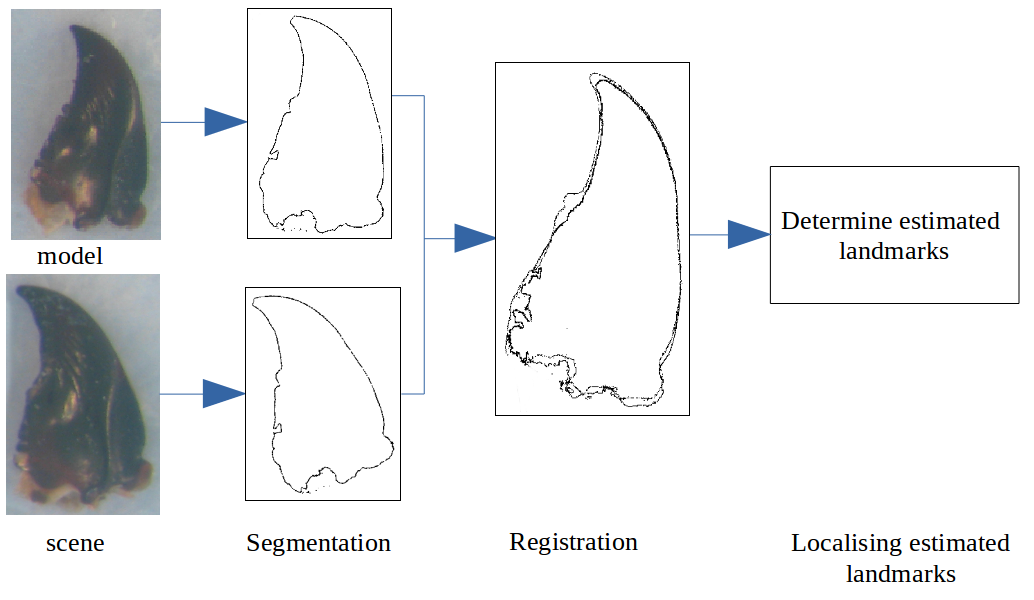
\includegraphics[width=0.48\textwidth]{./images/method}
    \caption{Overview of the proposed method.}
    \label{fig:method}
\end{figure}

\subsection{Image segmentation}
\label{sec:segmentation}

The segmentation step is the first task of a large number of image processing chains.
A contour-based algorithm, the Canny alogrithm \cite{canny1986computational}, has been chosen to extract the contour belonging to the shape of the mandible.
To use this method, two threshold values have to be set.
As it is mentioned in \cite{adaptiveCanny}, determine the right thresholds could be difficult.
The mandatory \textit{threshold value} is determined by analyzing the image histogram (see \cite{leestimating} for details).
Most often authors define these thresholds as a lower and an upper one with a usual ratio of $T_{lower} = (1/2) \times T_{upper}$.
In order to consider a larger range of values, we defined $T_{lower} = 1/3 \times T_{upper}$.
Note that to optimize the computing time, the direction of the gradient of each pixel belonging to the mandible contour is also computed during the Canny algorithm but will be used later (see Sec. \ref{sec:sift}).
To obtain the segmentation of the mandible, the contours obtained with Canny are discriminated to only keep the mandible contours.
As shown in Fig. \ref{canny}, the Canny algorithm generates some contours which do not belong to the mandible shape.
A simple algorithm parses the contour image to suppress the edges inside the biggest contour.

\begin{figure}[htbp]
\centering
\subfloat[Contours identified by the Canny algorithm.]
  {\label{canny1}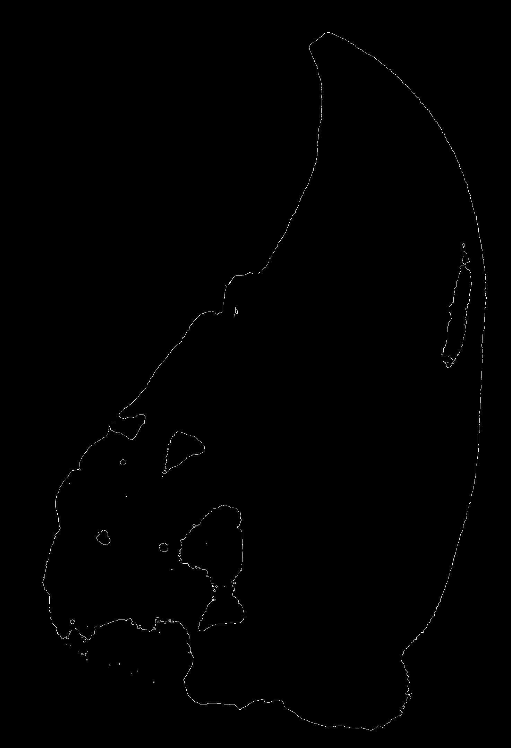
\includegraphics[width=0.23\textwidth]{./images/canny1}}~~
\subfloat[Contour selected by post-processing.]
  {\label{canny2}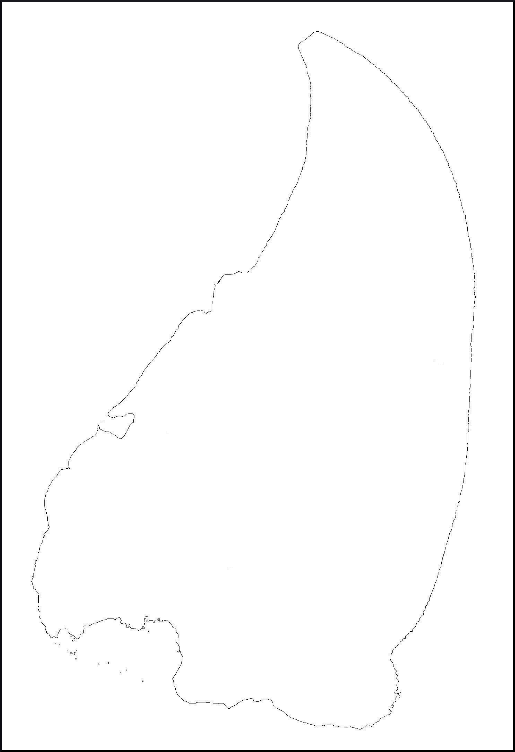
\includegraphics[width=0.23\textwidth]{./images/canny2}}
\caption{Detection of the mandible contours.}
\label{canny}
\end{figure}


\subsection{Image registration}
\label{sec:registration}

As previously mentioned, all images have been captured at the same scale.
However, the mandible size can may vary from a beetle to another one , as their orientation and position can differ from a picture to another one.
This point is take into account in this registration step from a query image (the scene) to a reference image (the model).

We have chosen to apply a method based on the Principal Component Analysis (PCA) \cite{bsspca,shlens2014tutorial} to determine the rotation and translation parameter between the two images.
In input, we consider the two lists of contour points defined from the segmentation of the two images.
Firstly, the centroid and the principal axis of each image are computed.
The centroid corresponds to the mean point of all contour points.
The principal axis is the line connecting the centroid to a contour point, determined with algorithm \ref{alg1}.

\begin{algorithm}
	\SetKwInOut{Input}{Input}
	\SetKwInOut{Output}{Output}
	\Input{Centroid $c$, list of contour points $l$}
	\Output{Principal axis $a$}
	\For{ all points $p_i$ in $l$ }
	{
		\For{ all points $p_j$ in $l$}
		{
			\If{$p_i \neq p_j$}
			{
				Compute the orthogonal distance $d_{ij}$ between the line $(c,p_i)$ and $p_j$.
			}
		}
		Compute $d_{mean}$ as the average distance of all $d_{ij}$ distances.\\

		\If{$d_{mean}$ is minimal}
		{
			$p_{min} = p_i$;\\
		}
	}
	The principal axis is: $a = (c,p_{min})$.
	\caption{Algorithm to find the principal axis of a list of contour points}
	\label{alg1}
\end{algorithm}

\begin{figure}[htbp]
    \centering
    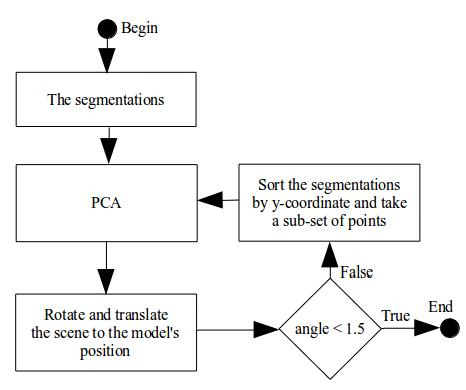
\includegraphics[width=0.48\textwidth]{./images/pcadiagram}
    \caption{Workflow of the PCAI, allowing to refine the rotation angle between the scene and the model.}
    \label{fig:pcai}
\end{figure}

The translation between the scene image and the model image is computed from the distance between their centroids.
The rotation is computed from the angle between the principal axes of these two images.
Translation then rotation operations are applied to register the scene on the model.
However the translation and rotation can be imprecise when the result of the segmentation contains noise.
In order to prevent these cases, we remarked and used the image specificity that implies that the tip of mandible is less noisy than its base.
So, we have sorted the contour points according to their y-value to build the subset containing the half upper part of contour points.
Then, we have enhanced the PCA by an Iterative process on this subset until stabilization (PCAI).
At each iteration, the rotation value is refined.
The procedure stop when the new computing angle is lower than $1.5$ degrees (see Fig. \ref{fig:pcai}).


The Fig. \ref{fig:box} shows an example of the successive results obtained with PCAI.
The red contours belongs to the model, the black one corresponds to the scene contour registered according the angle find after one iteration, and the blue contour is the
final contour obtained at the end of the PCAI process.

\begin{figure}[htbp]
    \centering
    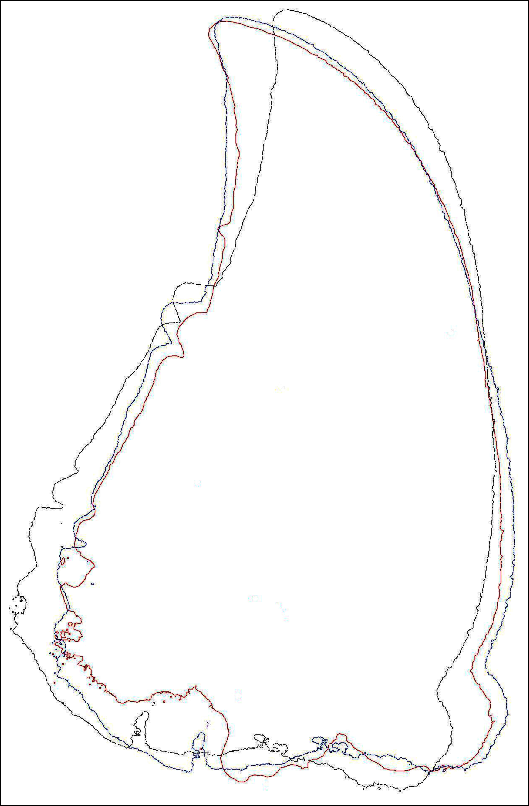
\includegraphics[width=.265\textwidth]{./images/imreg}
    \caption{Iterations of the registration step between the model contour (in red) and the contours of the scene image.}
    \label{fig:box}
\end{figure}

\subsection{Landmark detection with SIFT}
\label{sec:sift}

The last step of the workflow consists in estimating the position of the landmark in scene image from the manual ones of the model.
We relied on the SIFT method \cite{lowe2004distinctive} that has been used in a lot of computer vision methods to identify points of interests.
We modified some aspects of the initial method to defined a process specialized to the landmark identification.
In order to reduce the computing time and the possible errors of location, we do not consider all points of the image but only the area around each landmark on the model.
Firstly, the patch around each landmark of the model is computed and extracted at the same position in the scene image.
Then, the SIFT descriptor is computed.
The orientation and the gradient magnitude are calculated for each pixel by using the gradient values computed during contour detection (see Sec. \ref{sec:segmentation}) by applying the classical equations \ref{eq:sift}:

\begin{equation}
\label{eq:sift}
\begin{split}
	m_I(x,y) &= \sqrt{v_x^2 + v_y^2} \\
	\theta_I(x,y)& = tan^{-1}(v_y/v_x) \\
\end{split}
\end{equation}
Where:
\begin{itemize}[nosep,label=\footnotesize$\bullet$]
	\item $v_x = I(x+1,y) - I(x-1,y)$
	\item $v_y = I(x,y+1) - I(x,y-1)$
	\item $I(x,y)$ is the intensity of $I$ at position $(x,y)$,
	\item $m_I(x,y)$ is the gradient magnitude of in $I$ at position $(x,y)$,
	\item $\theta_I(x,y)$ is the orientation in $I$ at position $(x,y)$.
\end{itemize}

\begin{figure}[htbp]
    \centering
    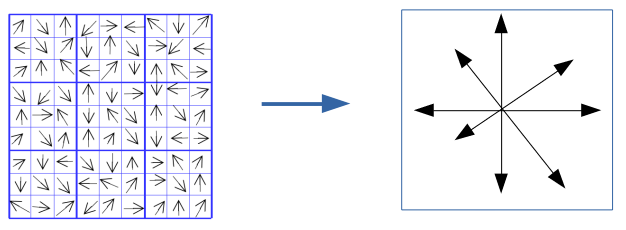
\includegraphics[width=0.48\textwidth]{./images/keypoint_descriptor}
    \caption{
        The SIFT descriptor of a patch.
        In the right figure, the arrow length corresponds to the gradient value.
    }
    \label{fig:kpdescriptor}
\end{figure}

For each patch, the SIFT descriptor is the histogram of the sum of gradients of each considered direction.
As usually, eight direction classes are considered : $[0^o-45^o[$, $[46^o-90^o[$, $[91^o-135^o[$, $[136^o-180^o[$, $[181^o-225^o[$, $[226^o-270^o[$, $[271^o-315^o[$, $[316^o-360^o[$).
The feature vector is normalized to reduce the effects of illumination changes.

The Fig. \ref{fig:kpdescriptor} shows a patch of $9\times9$ pixels centered in each landmark on the model.
The size of $9\times9$ has been retained after several tests where patch sizes $18\times18$, $36\times36$ and $54\times54$ have given unsatisfactory results.
From the histogram, we obtain the local gradient value for each direction.

The comparison between two SIFT descriptors is done by using the $L2$-distance with the following equation (\ref{eq:L2distance}):

\begin{equation}
\label{eq:L2distance}
	L(D1,D2) = \sum\limits_{i = 0}^{n}\sqrt{(D1_i-D2_i)^2}
\end{equation}
Where:
\begin{itemize}[nosep,label=\footnotesize$\bullet$]
	\item $n$ is the number of directions
	\item $D1$ and $D2$ are two descriptors of size $n$,
	\item $D1_i$ and $D2_i $ are the $i^{th}$ descriptor value.
\end{itemize}

The Fig. \ref{fig:Illustrate} illustrates how we have applied the SIFT method into our workflow.
IN order to detect the scene landmarks, the patches \textit{$P_m$} of the model and \textit{$P_s$} of the scene are initialized with the size of $P_m$ smaller than the size of $P_s$.
After experiments, we have kept $36 \times 36$ pixels as the size of \textit{$P_s$}.
For each pixel in the patch \textit{$P_s$}, a sub-patch \textit{$P'_s$} is extracted with the same size than \textit{$P_m$}.
When \textit{$P'_s$} have a part outside \textit{$P_s$}, the outside pixels are also considered.
Then, the distance \textit{$L(P_m,P'_s)$} is computed using equation (\ref{eq:L2distance}).
The estimated position of the landmark corresponds to the position of the sub-patch \textit{$P'_s$} with the smallest distance $L$ to \textit{$P_m$}.
Finally, the position of the estimated landmarks are positioned in the original scene image by applying the reverse operations of rotation and translation computed in registration step (see Sec. \ref{sec:registration}).

\begin{figure}[htbp]
    \centering
    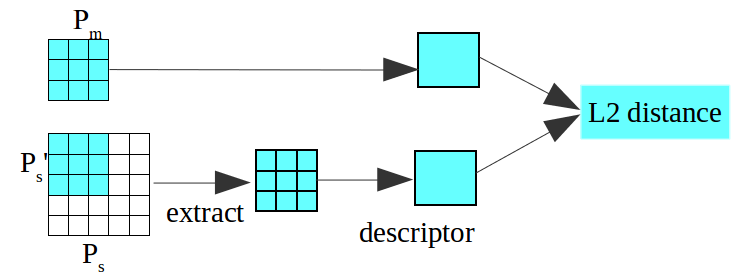
\includegraphics[width=0.48\textwidth]{./images/illustration_SIFT}
    \caption{Comparison of descriptors between the patch $P_m$ of the model image and the patches $P'_s$ of the scene image.}
    \label{fig:Illustrate}
\end{figure}

\section{Experiments and result}
\label{sec:experiments}

The complete method is implemented in the framework MAELab\footnote{MAELab
  is a free software written in C++. It can be directly and freely obtained by request
  at the authors.}. The left and the right mandibles of the beetles has been analyzed separately.
After verifying the quality of the image, it remains 290 usable images of right mandibles and 286 images of left mandibles.
The removed images include the images without mandible or with broken mandibles.
In all valid images, a set of manual landmarks is indicated by
biologists: 18 for right mandibles, 16 for left mandibles, which
constitutes our ground truth.

We have run the full workflow on all the usable images.
The results have shown differences in algorithm accuracy: estimated
landmarks are well positioned on some scene images but not satisfying
on others. As we mentioned before, mandibles images can exhibit
different sizes because beetles have also different sizes of
mandible. We detected that our method is sensible to this parameter.
To improve the results, we have inserted a pre-processing step to
estimate the scale between a scene image and the model before the
computing of the SIFT descriptors. The bounding boxes of the mandible
of the model image and the scene image are computed and the scales in the x-
and y-directions are determined by the ratio between the corresponding
sides of the bounding boxes. Then, the scene contours are rescaled to fit the model contours. \\
\begin{figure}[htbp]
\centering
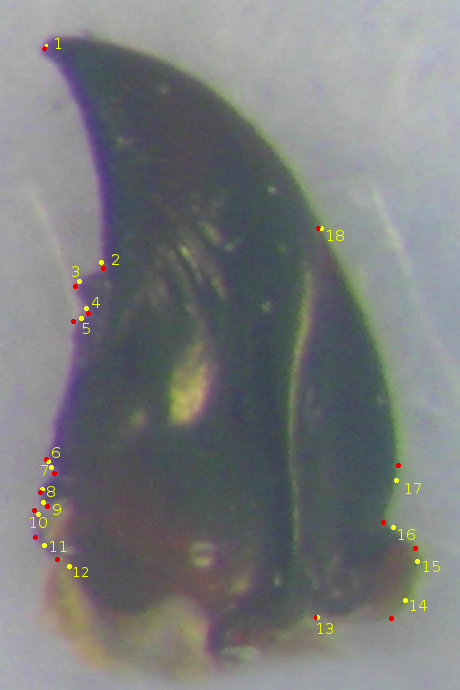
\includegraphics[width=0.35\textwidth]{./images/md_rs}
\caption{The manual (in red) and estimated (in yellow) landmarks on a right mandible.}
\label{figresult}
\end{figure}~\\
\begin{figure}[htbp]
\centering
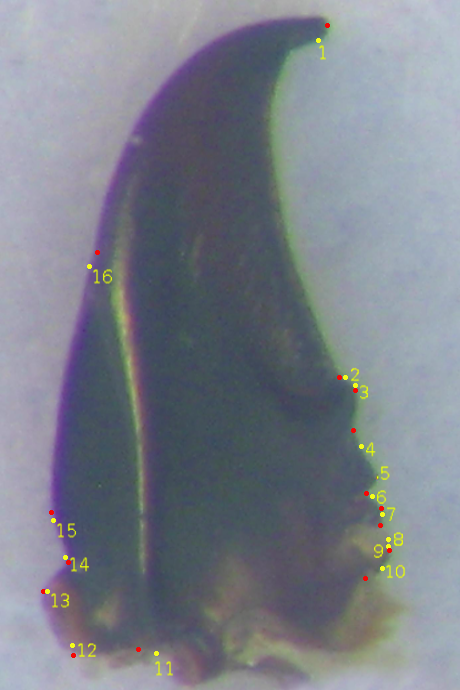
\includegraphics[width=0.35\textwidth]{./images/mg_rs}
\caption{The manual (in red) and estimated (in yellow) landmarks of a left mandible.}
\label{figresult2}
\end{figure}

Figs. \ref{figresult} and \ref{figresult2} show the final results
for a right and a left mandible with the manual and estimated
landmarks. The estimated landmarks are quite near with the manual
landmarks, as it is shown in the following statistical evaluation.
\\
The statistics have been computed for all landmarks of the scene images.
We have compared the positions between the manual and estimated
landmarks by accepting an error from 1\% to 2\% of the bounding box's
size. According to this way, a global statistic compares all pairs of
corresponding landmarks on all images as presented in
Fig. \ref{figctresult}. It shows the global results with a score of
well positioned landmarks equal to \textbf{87.03}\% for right
mandibles and \textbf{78.82}\% for left mandibles.

\begin{figure}[htbp]
\centering
\subfloat[Set of right mandibles.]{\label{figmdresult}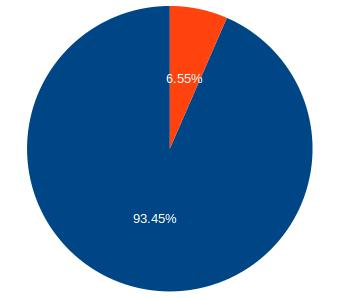
\includegraphics[width=0.22\textwidth]{./images/mdresult}}~~
\subfloat[Set of left mandibles.]{\label{figmgresult}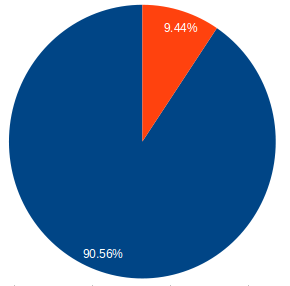
\includegraphics[width=0.22\textwidth]{./images/mgresult}}
\caption{The mean proportion of well and bad landmark locations of the two sets of left and right mandibles.}
\label{figctresult}
\end{figure}

Besides the global results, we are also interested by the accuracy of
the individual positions of the estimated landmarks.
We have computed the distance between the manual landmarks and their
corresponding estimated landmarks in order to examine the proportion
of well positioned landmarks. The Fig. \ref{figmdresultlm} and
\ref{figmgresultlm} show the proportion of well estimated landmarks
for each landmark of the model. With 18 landmarks of right mandible,
the position of the $1^{st}$ estimated landmarks is very accurate with
\textbf{98.62}\%. The lowest proportion is \textbf{74,48}\% for the
$14^{th}$ landmark. The remaining landmarks are also estimated with an
accuracy greater than 75\%. For left mandibles, the highest and lowest success rates are
\textbf{93,01}\% for the $1^{st}$ landmark and \textbf{60,14}\% for
the $16^{th}$ landmark. The statistic is done on each estimated
landmark of all the images with a standard deviation error
\cite{bland1996statistics}. As we can see in Fig. \ref{canny}, the
noise of the contour part located at the base of a mandible is higher
than the noise located at the tip of the mandible.
This explains why the correct proportion on $11^{th}$ and $12^{th}$
landmarks of the left mandible and $13^{th}$ and $14^{th}$ landmarks of
the right one are less accurate than other landmarks. Moreover,
when we reconsider the datasets, the left mandible images have bigger
scale values than the right mandible images. This could explain that the
success rate of the right mandibles is always greater than this one of the left
in all experiments.
\\
In  a previous work, we have tried to apply as set of procedures
coming from an article of Palaniswamy \cite{palaniswamy2010automatic} who tried to find
automatically a specific point of interest into a Drosophila wing. We
have successed to fix the centroid of the mandibles by using these
procedures (mainly based on the computation of a Probabilistic Hough
Transform accumulator). But this way has not been enough efficient to set
precisely the landmarks. D. Houle et al \cite{houle2003automated}
have more recently described a method to estimate automatically the
landmarks on Drosophila wings (with 12 landmarks). This method is
mainly based on the use of a curve analysis (with splines) belonging
to the wing shape. The method has been evaluated on 535 wing images.
The average proportion over all 12 points is 82\%. They have been able
to improve their results by suppressing the least accuracy point (47\%
of right results) that leads to a better parameter fitting. Y. Ke et
al. \cite{ke2004pca} have proposed to combine SIFT descriptor
with PCA analysis to characterize images belonging to a graffity
dataset. They also obtained good performances close to 95\% of correct
results. The results presented in this article can be considered as in
the same order of correctness than these works, but it concerns a problem, precise fixing of a
lot of landmarks, more difficult to solve. One can note that this chain of
treatments dedicated to the  estimation of landmarks on 2D images of
mandibles is from now, user friendly available.



\begin{figure}[htbp]
    \centering
    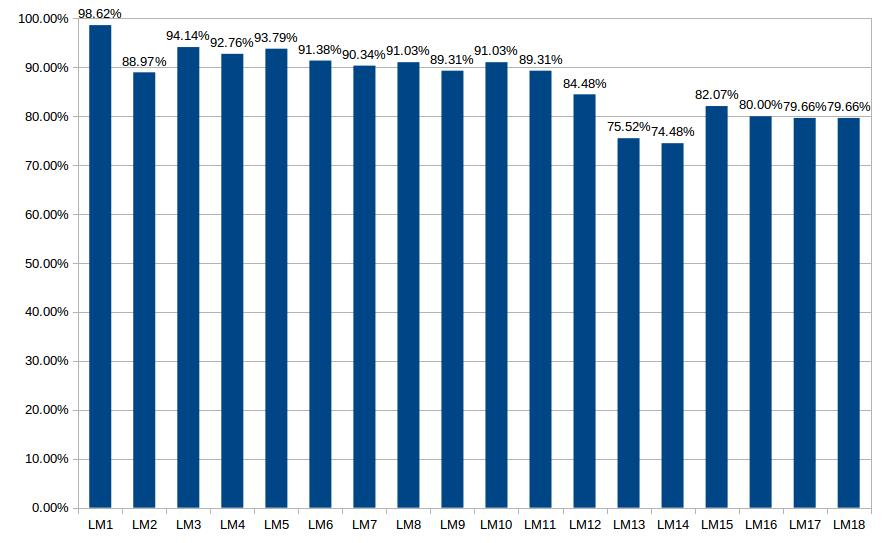
\includegraphics[width=0.5\textwidth]{./images/md_chartlms}
    \caption{The proportion of well estimated landmarks of right mandibles.}
    \label{figmdresultlm}
\end{figure}
\begin{figure}[htbp]
    \centering
    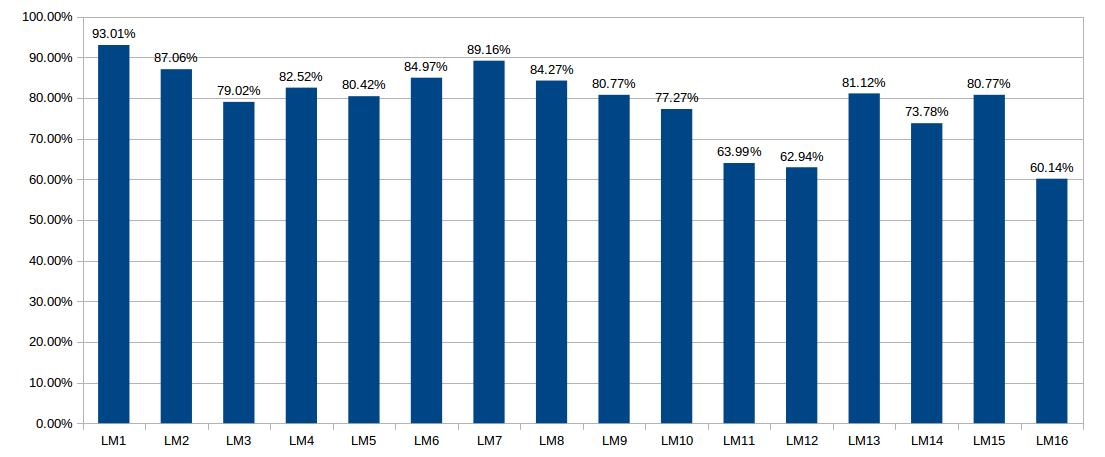
\includegraphics[width=0.5\textwidth]{./images/mg_chartlms}
    \caption{The proportion of well estimated landmarks of left mandibles.}
    \label{figmgresultlm}
\end{figure}

\section{Conclusion}

The morphometric analysis is a powerful tool to analyze and to
classify species. In this paper, we have designed a method to segment
the beetle mandibles and to automatically locate landmarks which have
been determined manually on an model image, by biologists. Each
mandible has been segmented by using the Canny algorithm before to be
registered using PCAI to align the images. The estimation step of the
landmark position use the SIFT descriptor to find the best matching
position.
The results show that the method succeed in locating the landmarks for all images.
The accuracy of the method is sufficient to be proposed to biologists
as an alternative to the manual measures. Moreover, considering the previous work in
\cite{leestimating}, this method reduces the drastically the number of
outlier landmarks and the MAELab implementation also reduce the global
computing times and memory cost. From now, the next stage consists in
improving the registration step in order to increase the matching step
accuracy and completely remove manual interventions. For example, we
could investigate deep learning methods, more precisely Convolutional
Neural Networks computing,  which have rised up in
image processing recently. Biologists are interested in large scale
analysis of their species collections, automatic classification is one of the
bottlenecks to solve towards a better integration of informatic procedures in
their current way to work.




\bibliographystyle{plain}
\bibliography{references}

\end{document}

Especially in agriculture, morphology is one of the best ways
to learn about the evolution of the beetle on crops


  They constitute
  the ground truth to evaluate the automatically estimated landmarks.



  If the goal is to consider more precisely
  the position or the geometry of the landmark areas, the results are not
   accurate enough to consider the replacement of manual landmarks by the automatically estimated landmarks. In this
   paper, we propose

Moreover, we
   have added a registration procedure based on an Iterative Principal Component Analysis.
   Finally, the landmarks are been located using a SIFT descriptor computed
   in the landmarks area of the model image and .

%-------------------------------------------------------------------------
% example of algorithm typesetting
% to allow this, uncomment line
% \RequirePackage[noend]{myalgorithm}
% in the wscg.sty file
% and download that package from Gabriel Zachmann's page http://zach.in.tu-clausthal.de/latex/
%
%
%\begin{algorithm}
%\hrule
%  \centering
%\begin{algorithmic}
%    \STMT $d_{l,r} = f_B(P_1), f_B(P_n)$
%    \WHILE{ $|d_l| > \epsilon $ and $|d_r| > \epsilon $ and $l<r$}
%        \STMT $d_x = f_B(P_x)$
%        \IF{ $d_x < 0$ }
%            \STMT $l, r = x, r$
%        \ELSE
%            \STMT $l, r = l, x$
%        \ENDIF
%    \ENDWHILE
%\end{algorithmic}
%\hrule
%\caption{Example of some pseudo-code}
%\label{fg:code}
%\end{algorithm}

%-------------------------------------------------------------------------

\begin{thebibliography}{99}
\label{references}
\bibitem[1]{canny} Canny, John. "A computational approach to edge detection." IEEE Transactions on pattern analysis and machine intelligence 6 (1986): 679-698.
\bibitem[2]{Ballard} Ballard, Dana H. "Generalizing the Hough transform to detect arbitrary shapes." Pattern recognition 13.2 (1981): 111-122.
\bibitem[3]{Webster} Webster, M. A. R. K., and H. DAVID Sheets. "A practical introduction to landmark-based geometric morphometrics." Quantitative Methods in Paleobiology 16 (2010): 168-188.
\bibitem[4]{est} Le Van, L., et al. "Estimating landmarks on 2D images of beetle mandibles."
\bibitem[5]{pca} Shlens, Jonathon. "A tutorial on principal component analysis." arXiv preprint arXiv:1404.1100 (2014).
\bibitem[6]{sift} Lowe, David G. "Distinctive image features from scale-invariant keypoints." International journal of computer vision 60.2 (2004): 91-110.
\bibitem[7]{palaniswamy} Palaniswamy, Sasirekha, Neil A. Thacker, and Christian Peter Klingenberg. "Automatic identification of landmarks in digital images." IET Computer Vision 4.4 (2010): 247-260.
\end{thebibliography}

%{\bfseries
%Last page should be fully used by text, figures etc. Do not leave empty space, please.

%Do not lock the PDF -- additional text and info will be inserted, i.e. ISSN/ISBN etc.
%}

%\begin{equation}
%\label{eq:sift}
%\resizebox{.5 \textwidth}{!}
%{$
%\begin{aligned}
%	m(x,y) = \sqrt{(P(x+1,y) - P(x-1,y))^2 + (P(x,y+1) - P(x,y-1))^2} \\
%	\theta(x,y) = tan^{-1}((P(x,y+1) - P(x,y-1))/(P(x+1,y) - P(x-1,y)))
%	\end{aligned}
%$}
%\end{equation}
